\documentclass{article}

\usepackage{graphicx} % Required for inserting images
\usepackage[left=1in,right=1in,top=1in,bottom=1in]{geometry} \usepackage{amsmath}
\usepackage{amsthm} %proof environment
\usepackage{amsthm} %proof environment
\usepackage{amssymb}
\usepackage{amsfonts}
\usepackage{enumitem} %nice lists
\usepackage{verbatim} %useful for something 
\usepackage{xcolor}
\usepackage{setspace}
\usepackage{titlesec}
\usepackage{blindtext} % I have no idea what this is 
\usepackage{caption}  % need this for unnumbered captions/figures
\usepackage{natbib}
\usepackage{appendix}
\usepackage{tikz}
\usepackage{hyperref}


\hypersetup{
    colorlinks=true,
    linkcolor=blue,
    filecolor=magenta,      
    urlcolor=blue,
    pdftitle={Overleaf Example},
    pdfpagemode=FullScreen,
    }

\titleformat{\section}{\bfseries\Large}{Problem \thesection:}{5pt}{}

\begin{document}

\title{AM 216 - Stochastic Differential Equations: Assignment 2}
\author{Dante Buhl}


\newcommand{\wrms}{w_{\text{rms}}}
\newcommand{\bs}[1]{\boldsymbol{#1}}
\newcommand{\tb}[1]{\textbf{#1}}
\newcommand{\bmp}[1]{\begin{minipage}{#1\textwidth}}
\newcommand{\emp}{\end{minipage}}
\newcommand{\R}{\mathbb{R}}
\newcommand{\C}{\mathbb{C}}
\newcommand{\N}{\mathcal{N}}
\newcommand{\Var}{\text{Var}}
\newcommand{\Cov}{\text{Cov}}
\newcommand{\Bino}{\text{Bino}}
\newcommand{\Norm}{\mathcal{N}}
\newcommand{\erf}{\text{erf}}
%\newcommand{\K}{\bs{\mathrm{K}}}
\newcommand{\m}{\bs{\mu}_*}
\newcommand{\s}{\bs{\Sigma}_*}
\newcommand{\dt}{\Delta t}
\newcommand{\dx}{\Delta x}
\newcommand{\tr}[1]{\text{Tr}(#1)}
\newcommand{\Tr}[1]{\text{Tr}(#1)}
\newcommand{\Div}{\nabla \cdot}
\renewcommand{\div}{\nabla \cdot}
\newcommand{\Curl}{\nabla \times}
\newcommand{\Grad}{\nabla}
\newcommand{\grad}{\nabla}
\newcommand{\grads}{\nabla_s}
\newcommand{\gradf}{\nabla_f}
\newcommand{\xs}{x_s}
\newcommand{\x}{\bs{x}}
\newcommand{\xf}{x_f}
\newcommand{\ts}{t_s}
\newcommand{\tf}{t_f}
\newcommand{\pt}{\partial t}
\newcommand{\pz}{\partial z}
\newcommand{\uvec}{\bs{u}}
\newcommand{\bvec}{\bs{B}}
\newcommand{\nvec}{\hat{\bs{n}}}
\newcommand{\tu}{\tilde{\uvec}}
\newcommand{\B}{\bs{B}}
\newcommand{\A}{\bs{A}}
\newcommand{\jvec}{\bs{j}}
\newcommand{\F}{\bs{F}}
\newcommand{\T}{\tilde{T}}
\newcommand{\ez}{\bs{e}_z}
\newcommand{\ex}{\bs{e}_x}
\newcommand{\ey}{\bs{e}_y}
\newcommand{\eo}{\bs{e}_{\bs{\Omega}}}
\newcommand{\ppt}[1]{\frac{\partial #1}{\partial t}}
\newcommand{\pp}[2]{\frac{\partial #1}{\partial #2}}
\newcommand{\pptwo}[2]{\frac{\partial^2 #1}{\partial #2^2}}
\newcommand{\ddtwo}[2]{\frac{d^2 #1}{d #2^2}}
\newcommand{\DDt}[1]{\frac{D #1}{D t}}
\newcommand{\ppts}[1]{\frac{\partial #1}{\partial t_s}}
\newcommand{\pptf}[1]{\frac{\partial #1}{\partial t_f}}
\newcommand{\ppz}[1]{\frac{\partial #1}{\partial z}}
\newcommand{\ddz}[1]{\frac{d #1}{d z}}
\newcommand{\ppzetas}[1]{\frac{\partial^2 #1}{\partial \zeta^2}}
\newcommand{\ppzs}[1]{\frac{\partial #1}{\partial z_s}}
\newcommand{\ppzf}[1]{\frac{\partial #1}{\partial z_f}}
\newcommand{\ppx}[1]{\frac{\partial #1}{\partial x}}
\newcommand{\ddx}[1]{\frac{d #1}{d x}}
\newcommand{\ppxi}[1]{\frac{\partial #1}{\partial x_i}}
\newcommand{\ppxj}[1]{\frac{\partial #1}{\partial x_j}}
\newcommand{\ppy}[1]{\frac{\partial #1}{\partial y}}
\newcommand{\ppzeta}[1]{\frac{\partial #1}{\partial \zeta}}
\renewcommand{\k}{\bs{k}}
\newcommand{\real}[1]{\text{Re}\left[#1\right]}


\maketitle 
% This line removes the automatic indentation on new paragraphs
\setlength{\parindent}{0pt}

\section{MLE and the Normal Distribution}
    
    Find $\mu_{(MLE)}$ and $\sigma_{(MLE)}$. 
    \begin{proof}
    \begin{align*}
        \ell(\mu, \sigma^2 | \bs{X}) &= -\frac{n}{2}\ln(2\pi) -
        \frac{n}{2}\ln(\sigma^2) - \frac{1}{2\sigma^2}\sum_{j=1}^n (X_j - \mu)^2
        \\
        \pp{\ell}{\mu} &= \frac{1}{\sigma^2}\sum_{i=1}^n (X_i-\mu)
        \\
        \mu_{(MLE)} &= \frac{1}{n}\sum_{i=1}^n X_i
        \\
        \pp{\ell}{\sigma^2} &= -\frac{n}{2\sigma^2} +
        \frac{1}{2\sigma^4}\sum_{i=1}^n (X_i - \mu)^2
        \\
        &= -\frac{n}{2\sigma^2} +
        \frac{1}{2\sigma^4}\sum_{i=1}^n (X_i - \frac{1}{n}\sum_{j=1}^n X_j)^2
        \\
        \sigma_{(MLE)} &= \sqrt{\frac{1}{n}\sum_{i=1}^n\left(X_i -
        \frac{1}{n}\sum_{j=1}^n X_j\right)^2}
    \end{align*}
    \end{proof}

\section{MLE Variance and unbiased sample variance}
    Show that the MLE of variance is biased. 
    \begin{proof}
        \begin{align*}
            E\left(\sum_{i=1}^n \left(X_i - \frac{1}{n}\sum_{j=1}^n
            X_j\right)^2\right) &= \sum_{i=1}^n E\left(\left(X_i -
            \frac{1}{n}\sum_{j=1}^n
            X_j\right)^2\right)
            \\
            &= \sum_{i=1}^n \Var\left(X_i -
            \frac{1}{n}\sum_{j=1}^n X_j\right) + \left(E\left(X_i -
            \frac{1}{n}\sum_{j=1}^n X_j\right)\right)^2
            \\
            E\left(X_i -
            \frac{1}{n}\sum_{j=1}^n X_j\right) &= E(X_i) +
            \frac{1}{n}\sum_{j=1}^n E(X_j)
            \\
            &= \mu + \frac{1}{n}n\mu
            \\
            &= 0 
            \\
            \Var\left(X_i -
            \frac{1}{n}\sum_{j=1}^n X_j\right) &= 
            \Var(X_i) + \Var(\mu) - 2\Cov(X_i,\mu)
            \\
            &= \sigma^2 + \frac{1}{n}\sigma^2 -
            \frac{2}{n}\sigma^2
            \\
            &= \left(1-\frac{1}{n}\right)\sigma^2
            \\
            E\left(\sum_{i=1}^n \left(X_i - \frac{1}{n}\sum_{j=1}^n
            X_j\right)^2\right) &= \sum_{i=1}^n \left(1 -
            \frac{1}{n}\right)\sigma^2
            \\
            &= (n-1)\sigma^2
            \\
            &= (n-1)\Var(X)
        \end{align*}
    \end{proof}

\section{Central Limit Theorem}
    \begin{enumerate}[label=\roman*)]
        \item 
            \begin{align*}
                \phi_X(\xi) &= \int_{-\infty}^{\infty} e^{i\xi x}f(x)dx 
                \\
                &= pe^{i\xi} + q
            \end{align*}
        \item 
            \begin{align*}
                \phi_N(\xi) &= \int_{-\infty}^{\infty} e^{i\xi x}f(x)dx 
                \\
                &= \sum_{k=0}^n \left(\begin{array}{c} n\\k\end{array}\right)
                p^k(1-p)^{n-k}e^{i\xi k}
            \end{align*}
        \item 
            \begin{align*}
                \phi_Y(\xi) &= \phi_N(\xi/\sqrt{n})\exp(i\xi\sqrt{n}p)
                \\
                &= \sum_{k=0}^{n} \left(\begin{array}{c} n\\k +
                np\end{array}\right)
                p^{k}(1-p)^{n-k}e^{i\xi\left(\frac{k}{\sqrt{n}}+\sqrt{n}p\right)}
            \end{align*}
        \item
            \begin{align*}
                \lim_{n\to\infty} \phi_Y(\xi) &= 
                \lim_{n\to\infty}\sum_{k=0}^{n} \left(\begin{array}{c} n\\k +
                np\end{array}\right)
                p^{k}(1-p)^{n-k}e^{i\xi\left(\frac{k}{\sqrt{n}}+\sqrt{n}p\right)}
            \end{align*}
            My proof ends here, I have not figured out how to pull an extra
            $\xi$ out of the PMF function and obtain a $e^{\xi^2(\cdots)}$. As
            such, I will resubmit this assignment once I have solved this
            particular problem. 
    \end{enumerate}

\section{Sample Variance v.s. MLE variance}
    See Figure \ref{fig:p4}
    \begin{figure}[ht]
        \centering
        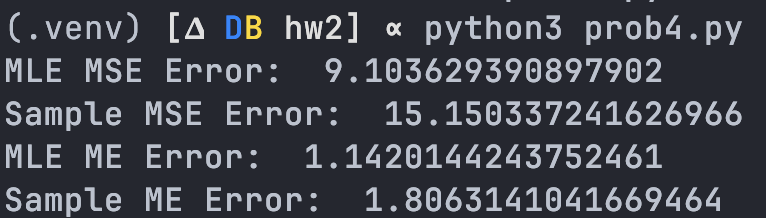
\includegraphics[width=\textwidth]{prob4.png}
        \caption{Results from problem 4}
        \label{fig:p4}
    \end{figure}
    Generally we find that minimizing the fluctuations (using the MLE
    variance) decreases the error in estimating the distributions
    variance as opposed to minimizing the bias (using the sample
    variance). 

\section{Deriving the CF of a multivariate gaussian}
    \begin{proof}
        {\small
        \begin{align*}
            i\xi^Tx - \frac{1}{2}(x - \mu)^T \Sigma^{-1}(x-\mu) &=
            -\frac{1}{2}\left(x - \mu - i\Sigma\xi\right)^T\Sigma^{-1}\left(x -
            \mu - i\Sigma\xi\right) + \left(i\xi^T\mu -
            \frac{1}{2}\xi^T\Sigma\xi\right)
            \\
            i\xi^Tx &=
            -\frac{1}{2}\left[-i(x - \mu)^T\Sigma^{-1}\Sigma\xi + 
            -i\xi^T\Sigma^T\Sigma^{-1}(x - \mu) -
            \xi^T\Sigma^T\Sigma^{-1}\Sigma\xi\right]
             + \left(i\xi^T\mu -
            \frac{1}{2}\xi^T\Sigma\xi\right)
            \\
            &= \frac{i}{2}(x-\mu)^T\xi + \frac{i}{2}\xi^T(x-\mu)  + i\xi^T\mu
            \\
            &= i\xi^Tx
        \end{align*}
        }
        where here the symmetry of the inner product operator satisfies the
        movement between the third and fourth lines and its distributive
        properly allows the movement between the 1st and 2nd lines. 
    \end{proof}

\section{Deriving the Conditional Gaussian Distribution}
    \begin{proof}
        \begin{gather*}
            \Sigma = \left[\begin{array}{c c} \Sigma_{XX} & \Sigma_{XY} \\
               \Sigma_{YX} & \Sigma_{YY}\end{array}\right], \quad\quad
                \Sigma^{-1} = \left[\begin{array}{c c} A & B \\
                B^T & C\end{array}\right]
                \\
                \Sigma^{-1}\Sigma = I
                \\
                \left[\begin{array}{c c}
                A\Sigma_{XX} + B\Sigma_{YX} & A\Sigma_{XY} + B\Sigma_{YY}\\
                B^T\Sigma_{XX} + C\Sigma_{YX} & B^T\Sigma_{XY} + C\Sigma_{YY}
                \end{array}\right] = \left[\begin{array}{c c} I & 0 \\ 0 &
                I\end{array}\right]
                \\
                A\Sigma_{XY} + B\Sigma_{YY} = 0
                \\
                -A\Sigma_{XY} =  B\Sigma_{YY}
                \\
                -\Sigma_{XY}\Sigma_{YY}^{-1} = A^{-1}B
                \\
                A\Sigma_{XX} + B\Sigma_{YX} = 0 
                \\
                A\left(\Sigma_{XX} -
                \Sigma_{XY}\Sigma_{YY}^{-1}\Sigma_{YX}\right) = I
                \\
                A^{-1} = \left(\Sigma_{XX} -
                \Sigma_{XY}\Sigma_{YY}^{-1}\Sigma_{YX}\right)
        \end{gather*}
    \end{proof}

\section{Random Monty Hall's Game}
    \begin{proof}
        In order to make this decision we must look at the conditional
        probabiliites involved with the random variant of the Monty Hall's game.
        In this problem, we study the conditional probability $Pr(X|Y =
        \text{empty})$ where
        $X$ is the box we first chose and $Y$ is the box that we first open. 
        We have using Bayes Theorem, 
        \begin{align*}
            Pr(X|Y) &= \frac{Pr(Y|X)Pr(X)}{Pr(Y)}
            \\
            &= \frac{(1)(1/3)}{2/3} 
            \\
            &= \frac{1}{2}
        \end{align*}
        As we can see from this, since we are not guaranteed that the host
        reveals an empty box, we no longer have an advantage from switching. 
    \end{proof}

\section{Finite Difference Equation}

    \begin{enumerate}[label=\roman*)]
        \item See Fig \ref{fig:p8pa}
            \begin{figure}[ht]
                \centering
                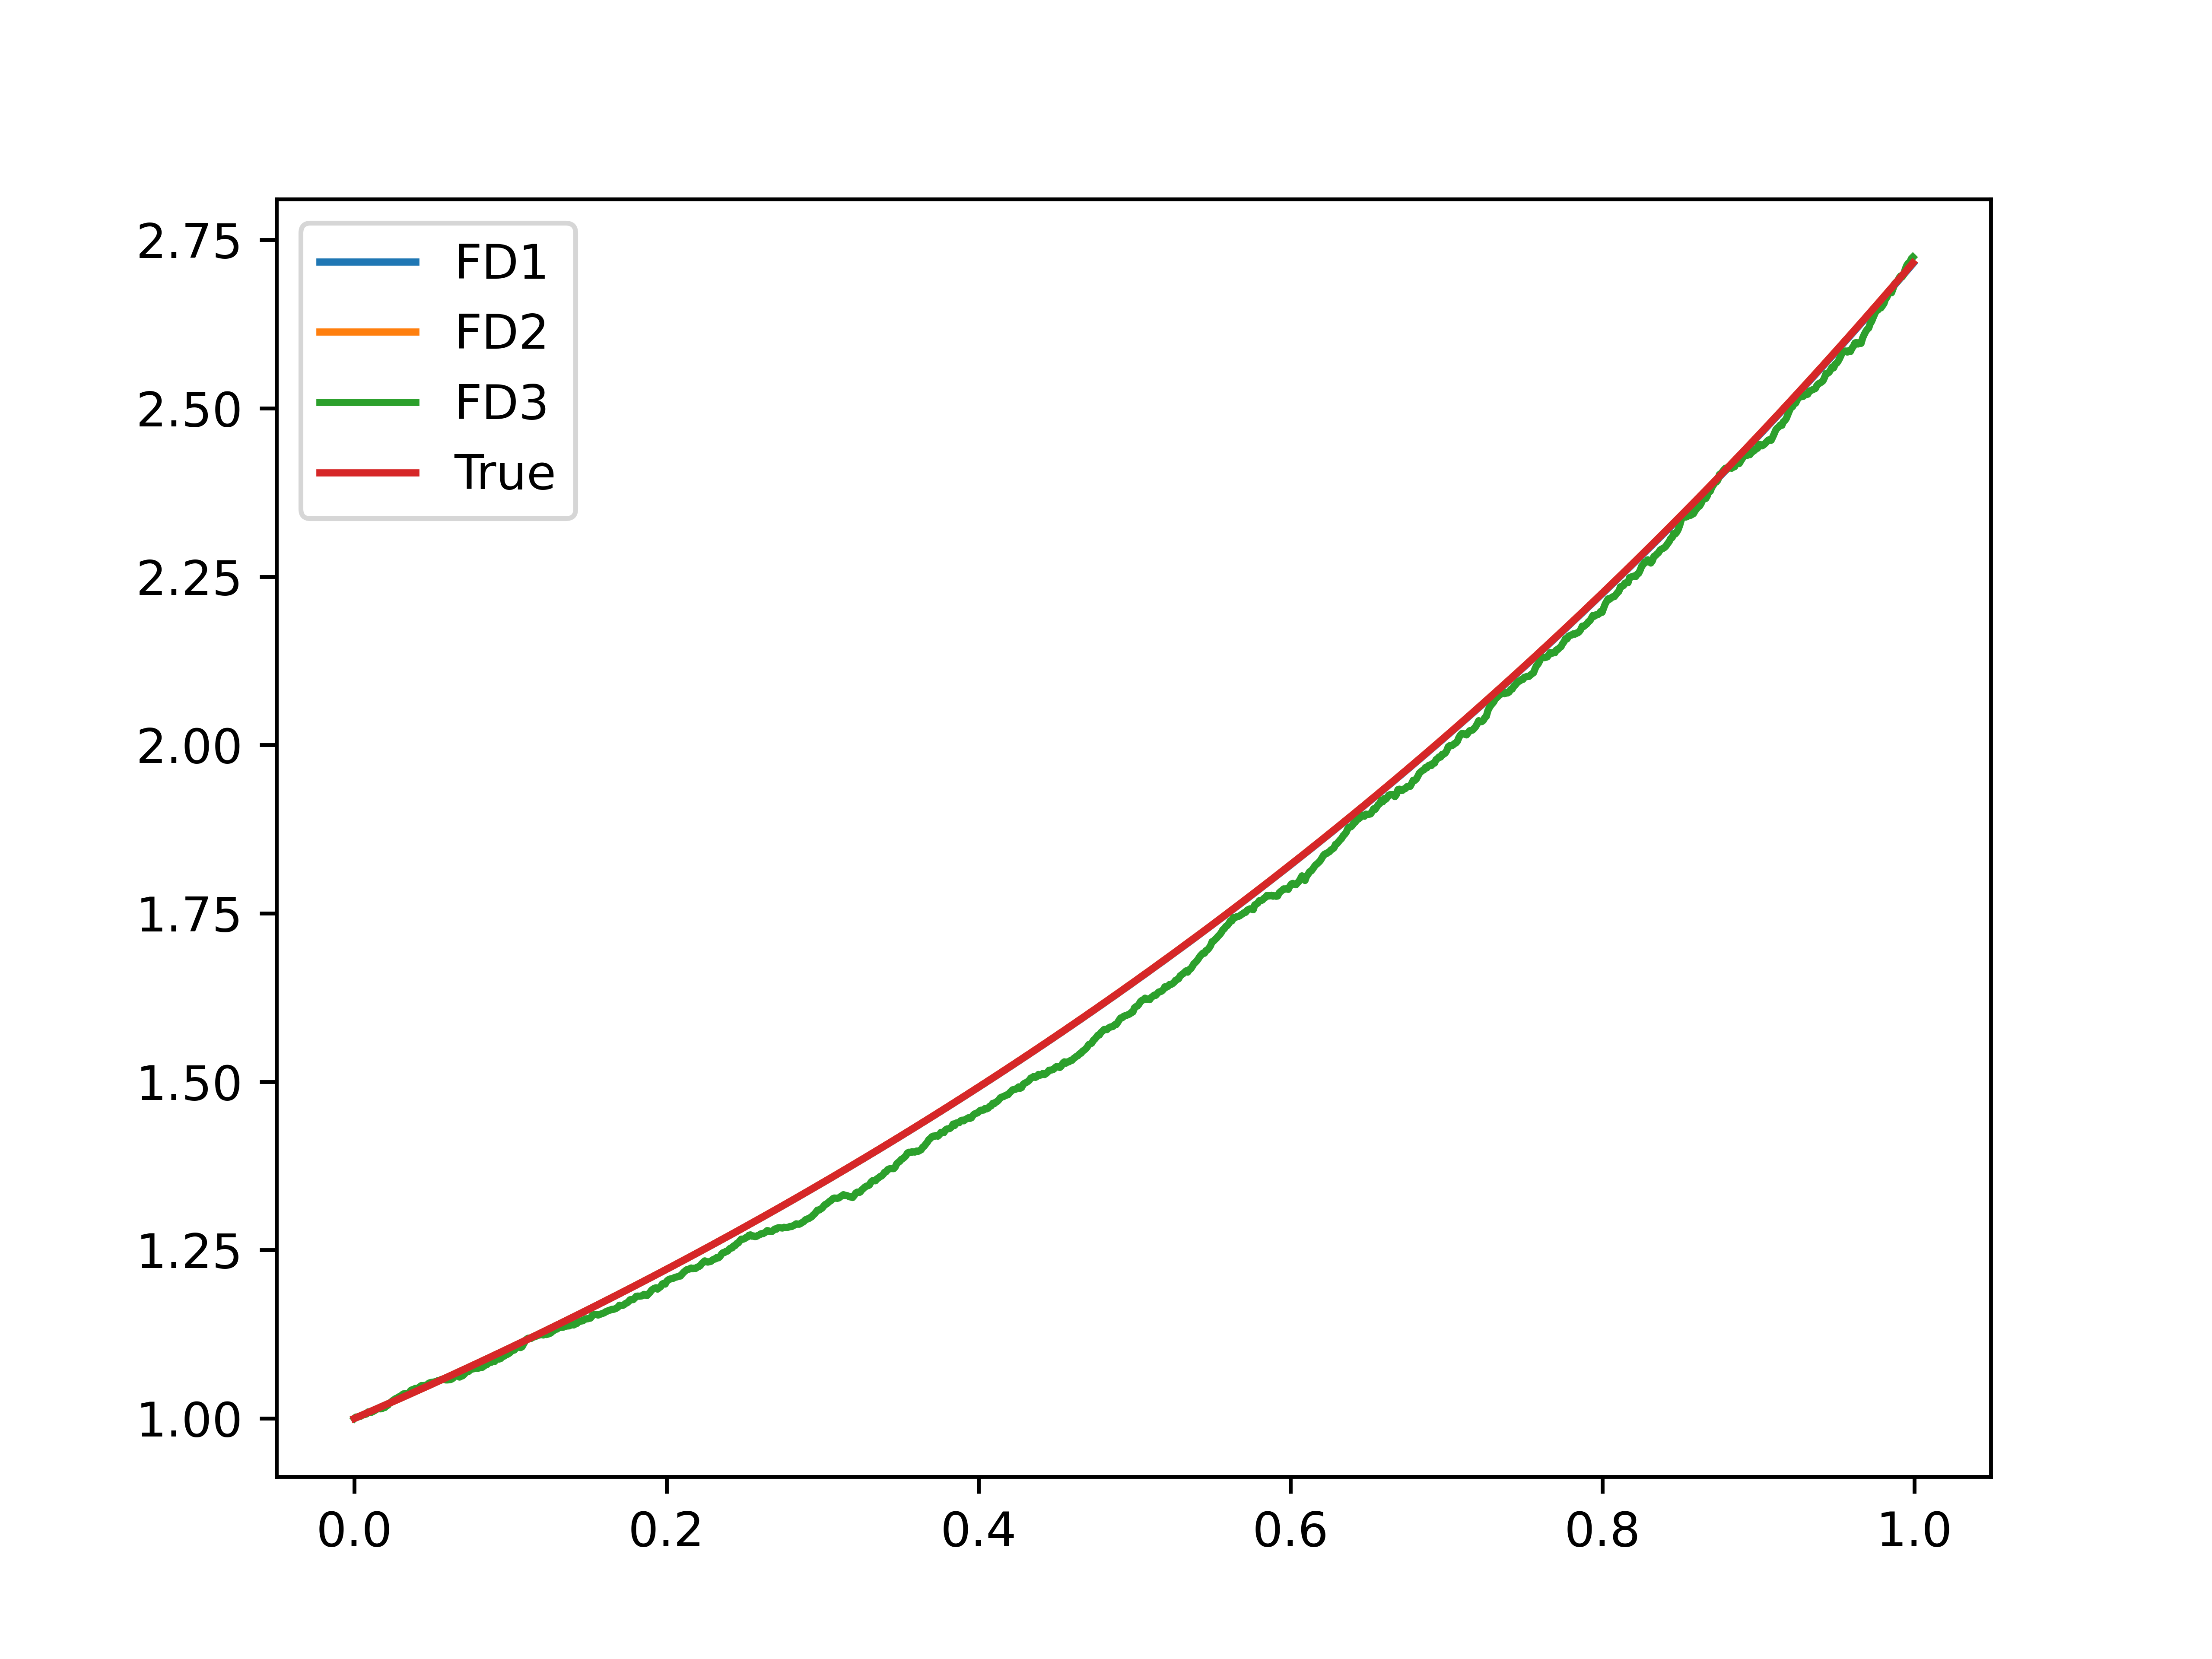
\includegraphics[width=\textwidth]{prob8_parta.png}
                \caption{P8 Part a}
                \label{fig:p8pa}
            \end{figure}
        \item See Fig \ref{fig:p8pb}
            \begin{figure}[ht]
                \centering
                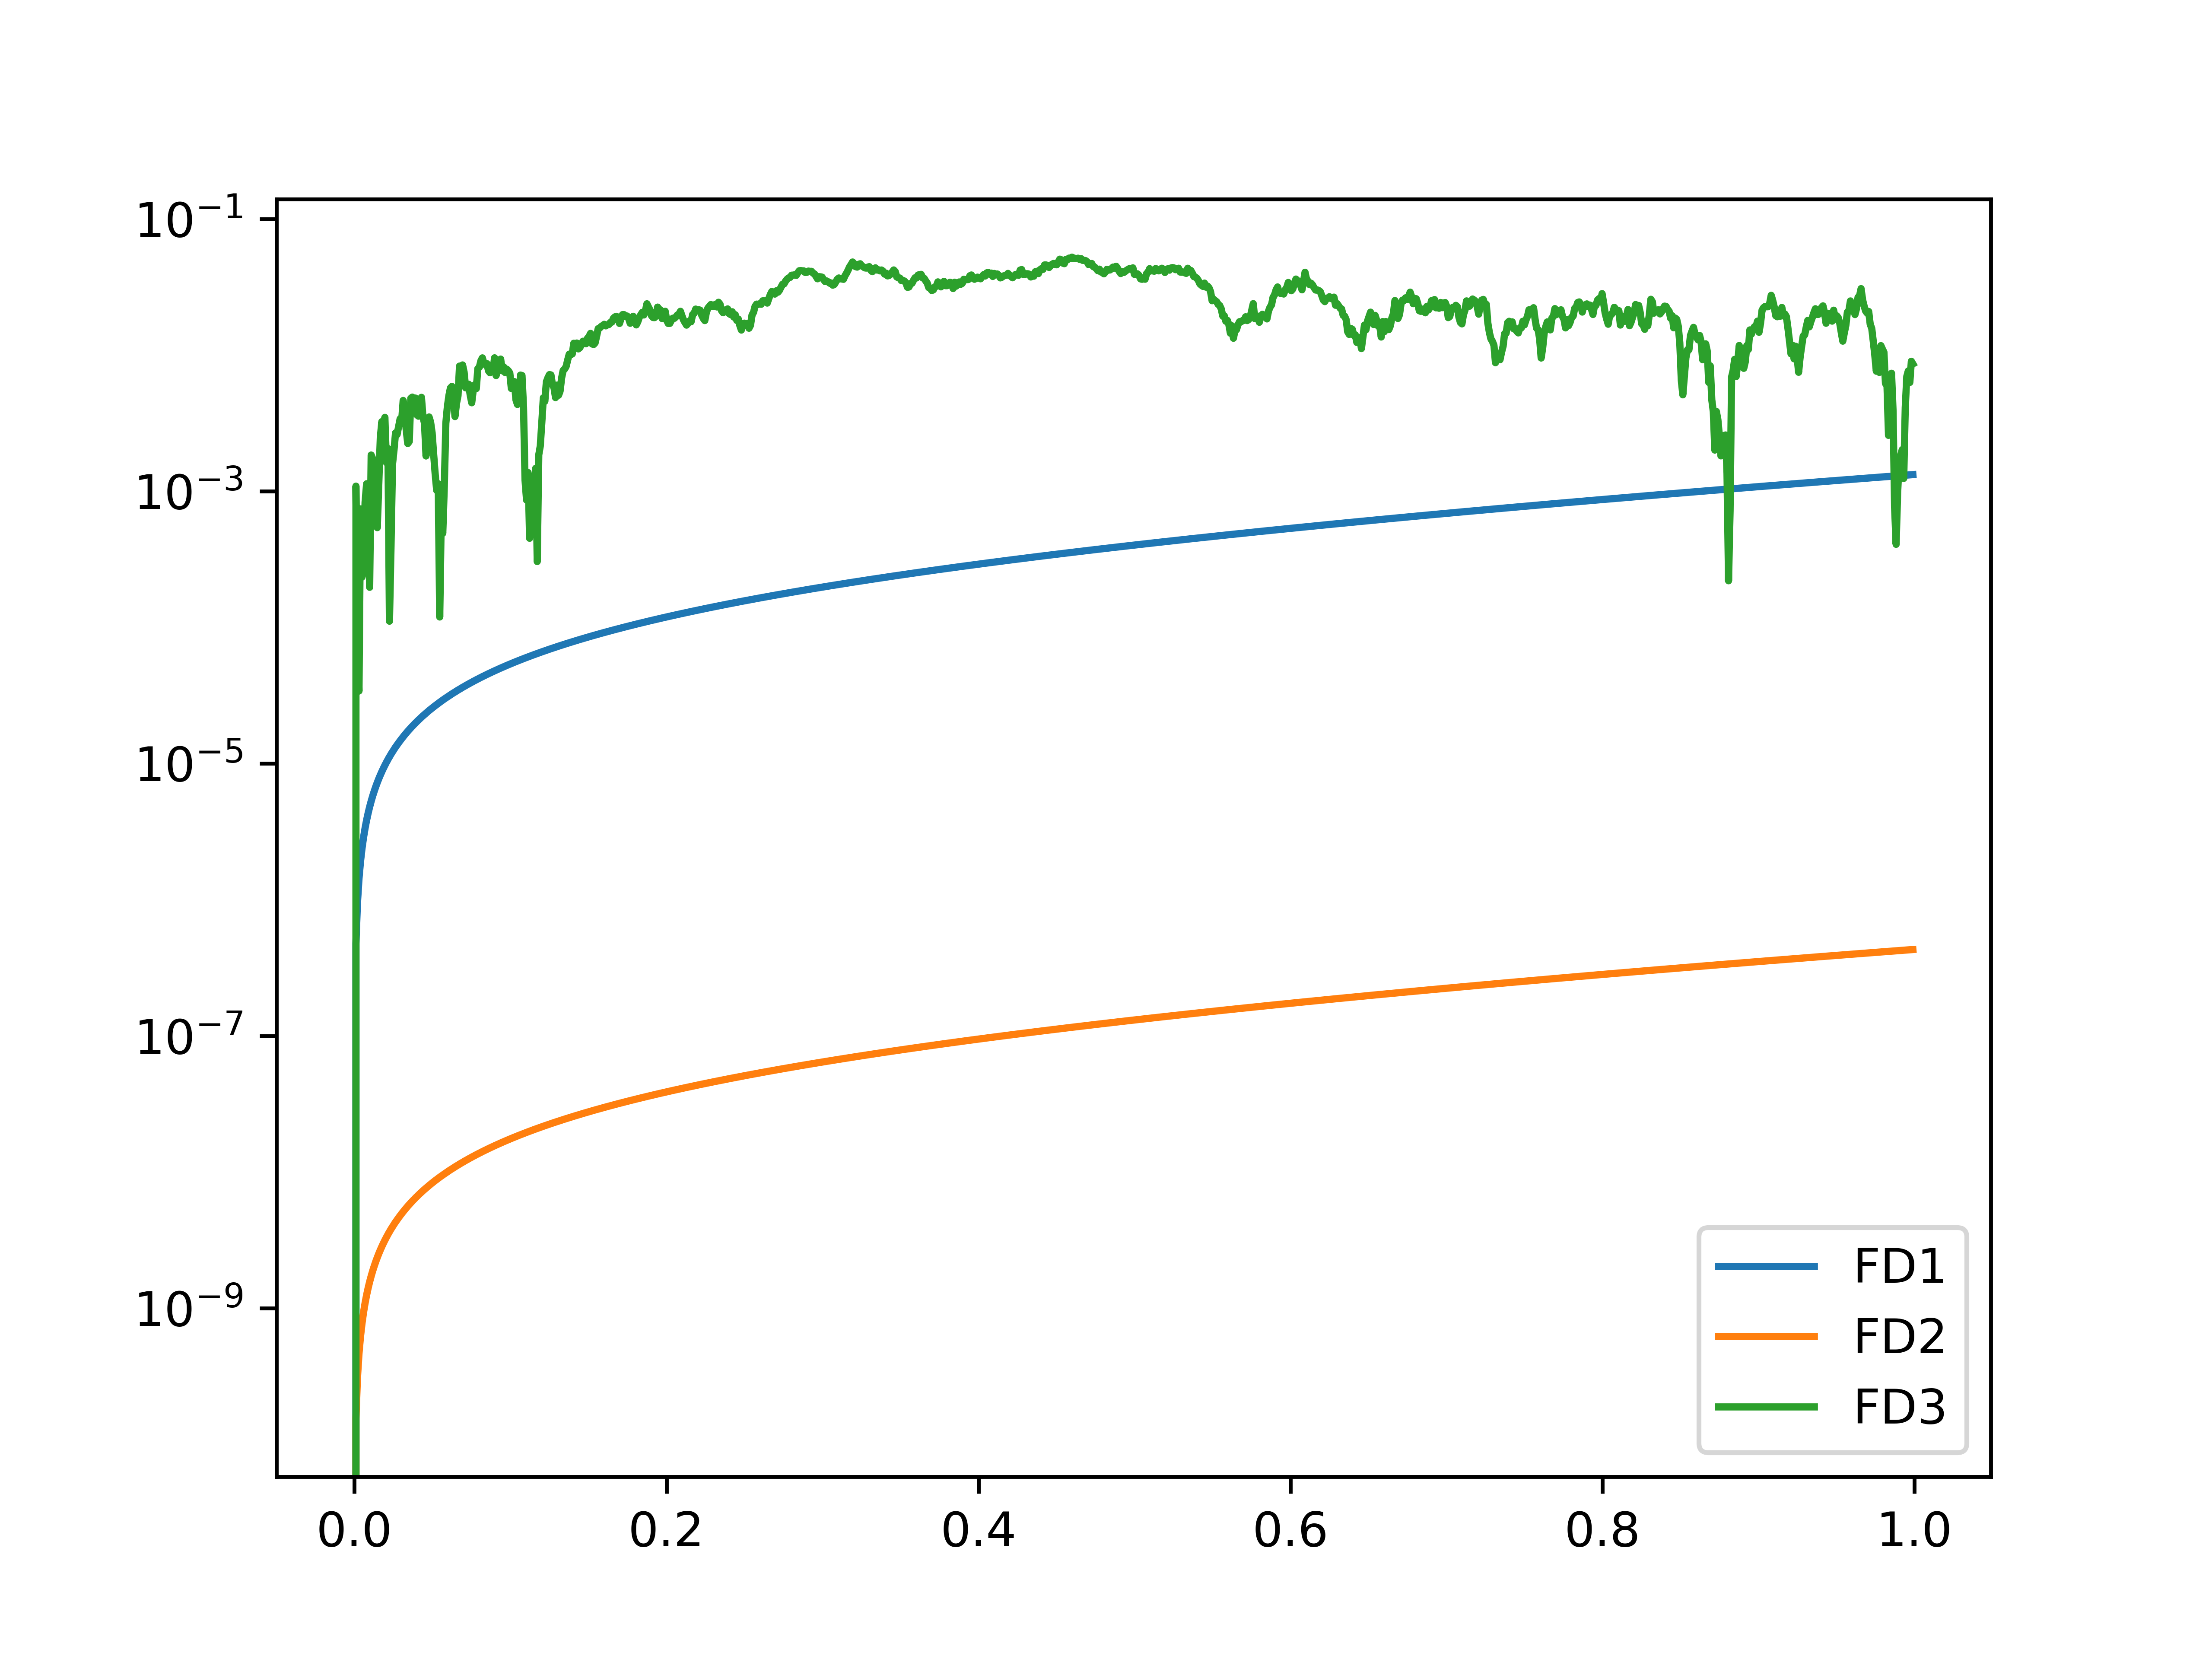
\includegraphics[width=\textwidth]{prob8_partb.png}
                \caption{P8 Part b}
                \label{fig:p8pb}
            \end{figure}
        \item See Fig \ref{fig:p8pc}
            \begin{figure}[ht]
                \centering
                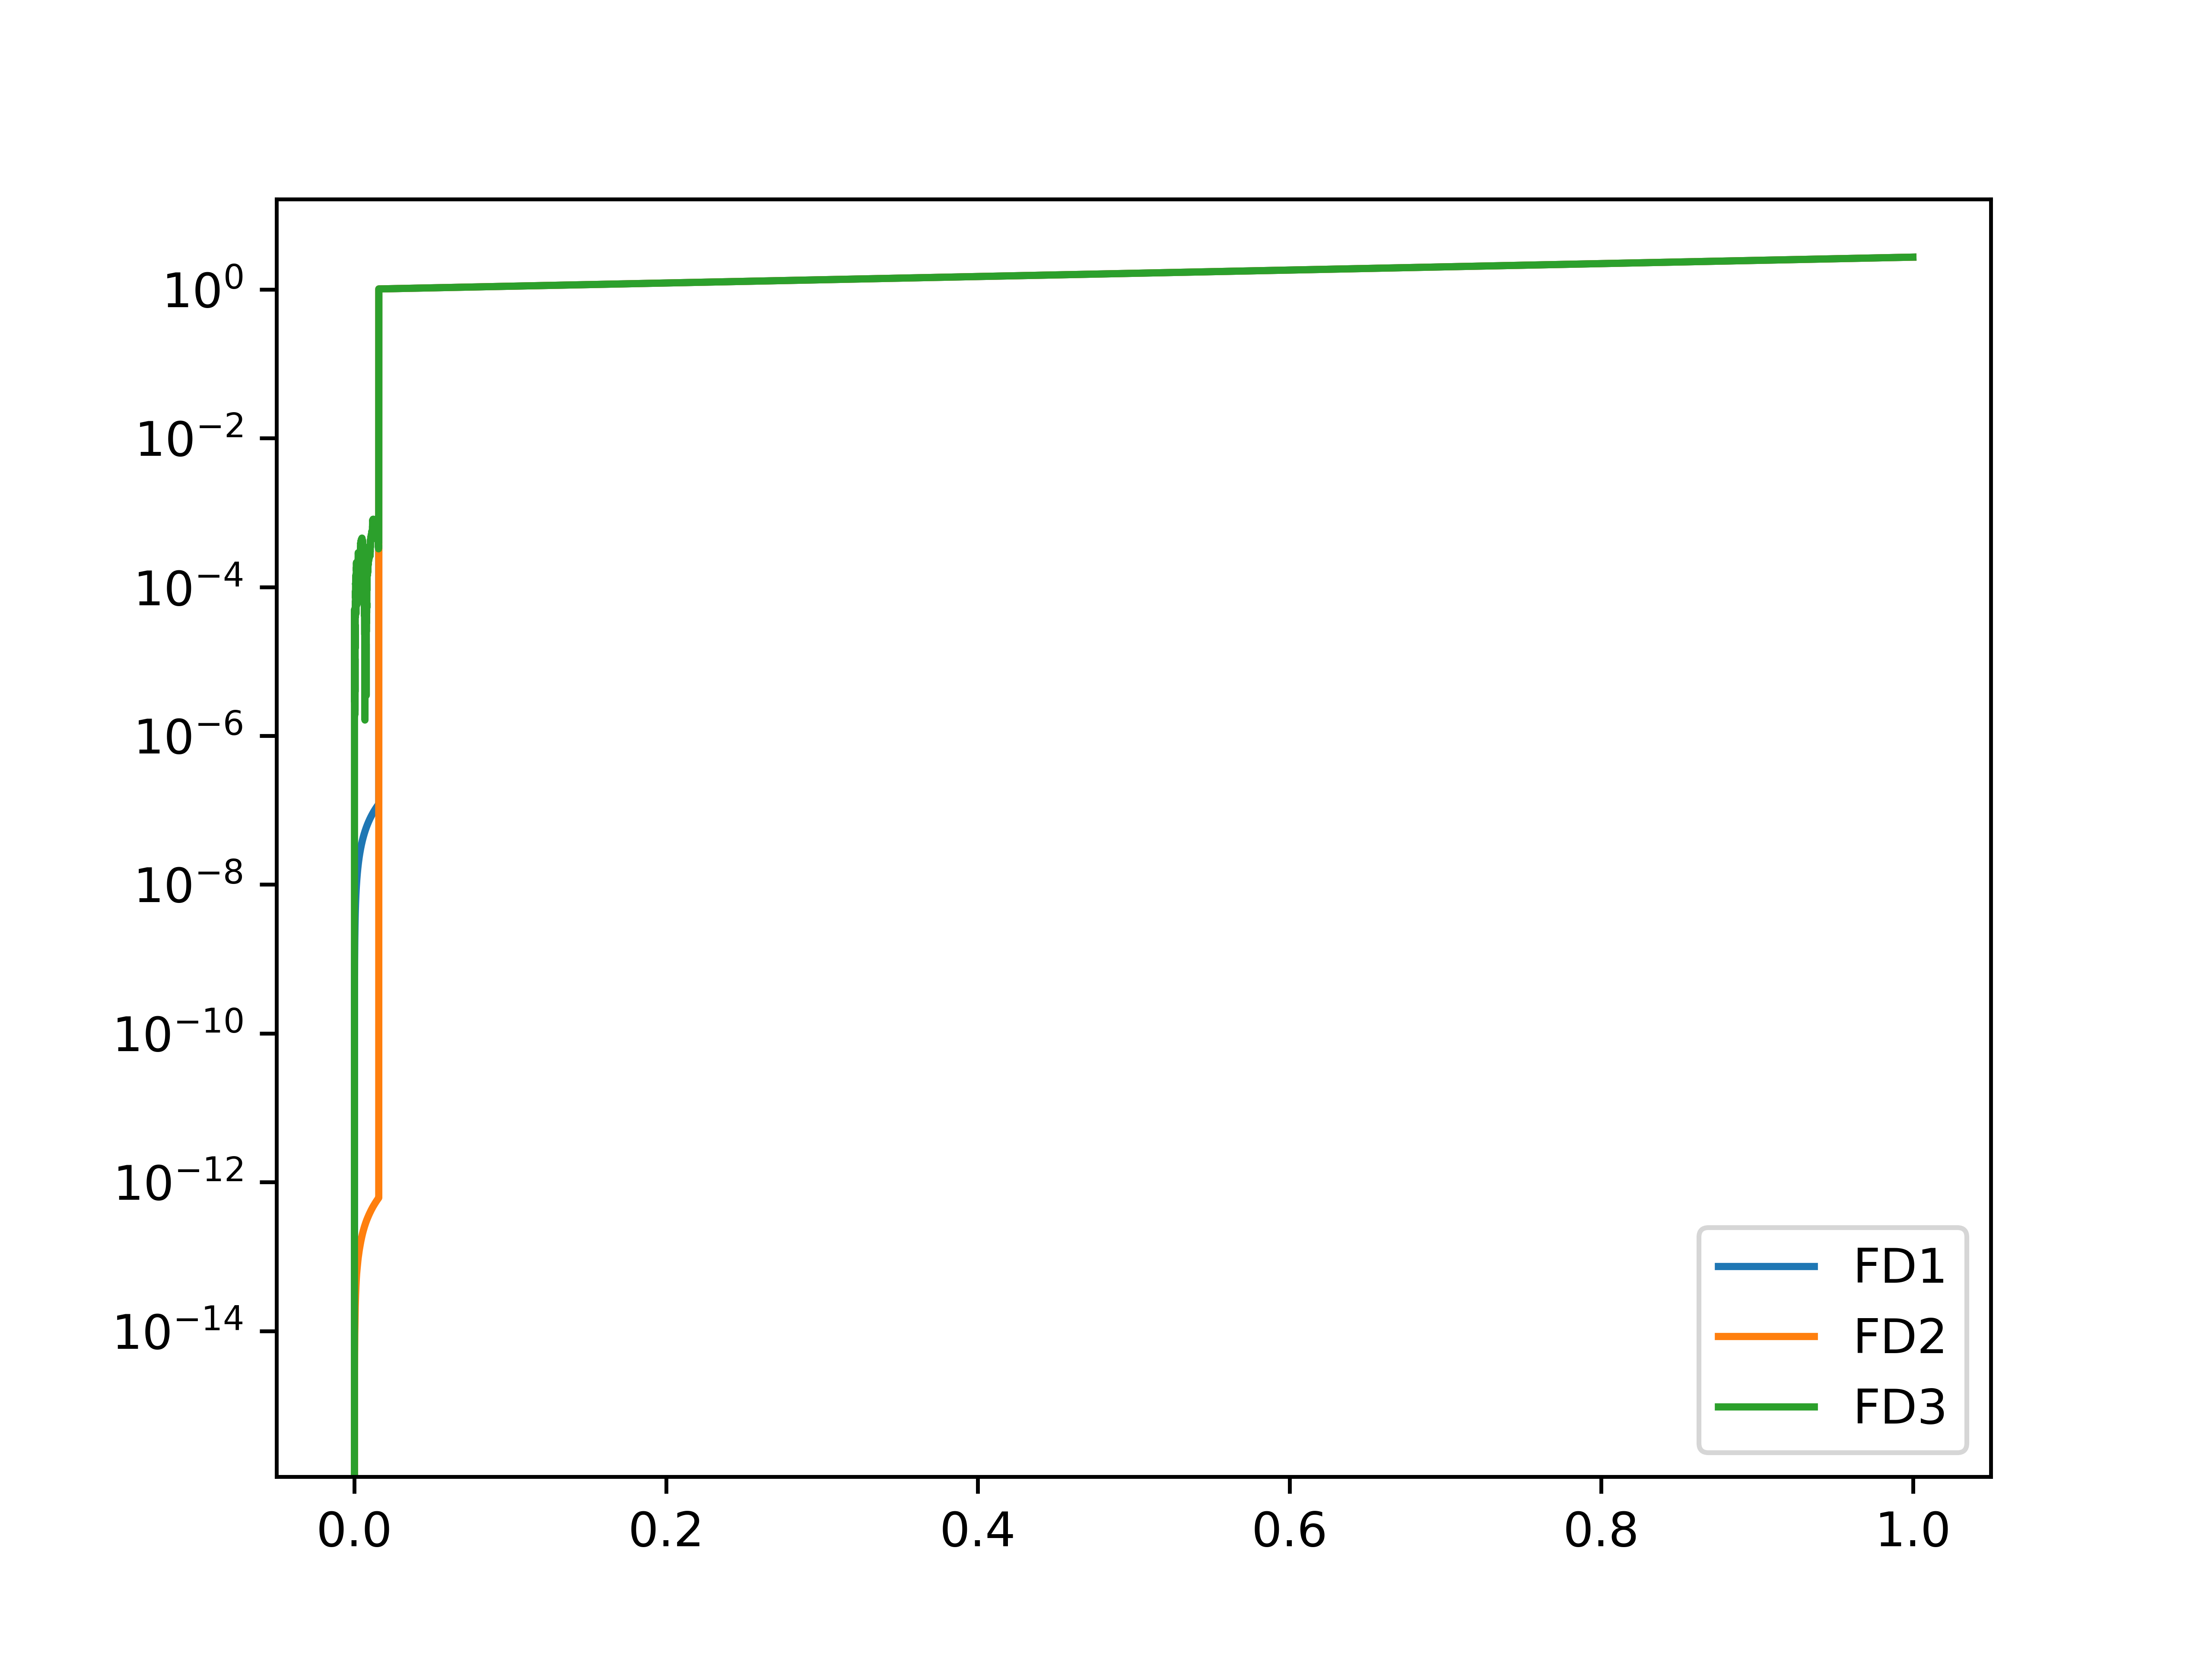
\includegraphics[width=\textwidth]{prob8_partc.png}
                \caption{P8 Part c}
                \label{fig:p8pc}
            \end{figure}

    \end{enumerate}
    

\end{document}
